\documentclass[tikz,border=5pt]{standalone}
\usepackage{tikz}
\usepackage{amsmath}
\usetikzlibrary{arrows.meta}
\definecolor{nebula}{HTML}{6366F1}
\definecolor{spark}{HTML}{14B8A6}
\definecolor{ink}{HTML}{334155}
\begin{document}
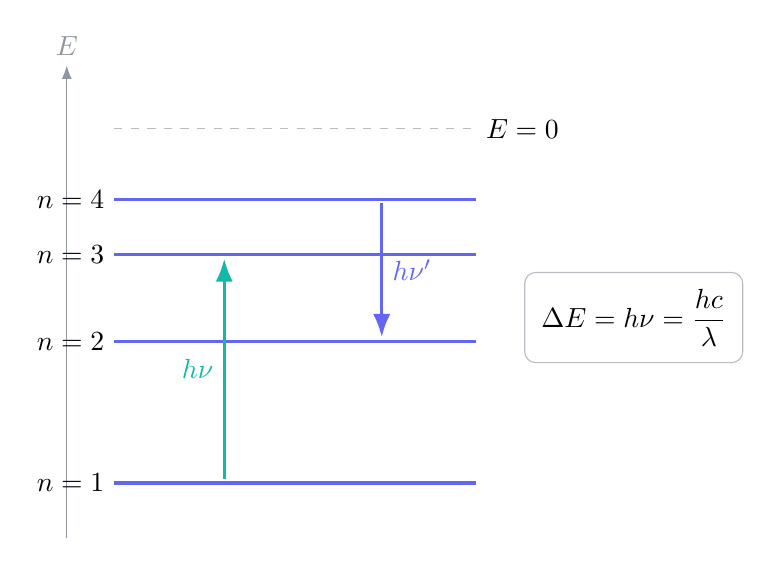
\begin{tikzpicture}[font=\sffamily,>=Latex,x=1cm,y=1cm]
  \draw[->,ink!55] (0,0)--(0,6) node[above] {$E$};
  \foreach \y/\n in {.7/1,2.5/2,3.6/3,4.3/4} {
    \draw[very thick,nebula] (.6,\y)--(5.2,\y);
    \node[left] at (.6,\y) {$n=\n$};
  }
  \draw[dashed,ink!35] (.6,5.2)--(5.2,5.2);
  \node[right] at (5.2,5.2) {$E=0$};
  \draw[->,very thick,spark] (2.0,.75)--(2.0,3.55) node[midway,left] {$h\nu$};
  \draw[->,very thick,nebula] (4.0,4.25)--(4.0,2.55) node[midway,right] {$h\nu'$};
  \node[draw=ink!35,rounded corners=4pt,fill=white,inner sep=6pt] at (7.2,2.8) {$\Delta E=h\nu=\dfrac{hc}{\lambda}$};
\end{tikzpicture}
\end{document}
